%MSc template Version 1.0.2
%this version adds version numbering, candidate number and changes referencing style
%and corrections/comments/requests, please email alastair.kay@rhul.ac.uk
\documentclass[11pt,twoside]{report}
%this is a comment, and does nothing.

%import useful packages here
\usepackage{amsfonts,amssymb,amsmath}            % for math symbols.
\usepackage{lmodern}
\usepackage[]{graphics,graphicx}            % for graphics figures.
\usepackage{amsthm}
\usepackage[utf8]{inputenc}
\usepackage{caption}
\usepackage{subcaption}
\usepackage[a4paper,width=150mm,top=25mm,bottom=25mm,bindingoffset=6mm]{geometry}
\usepackage{fancyhdr}
%\usepackage[Lenny]{fncychap}	%This is a way of doing pretty starts to chapters. I like Bjarne or Lenny as options
\usepackage{hyperref}			%Lets you have links in your document
\usepackage[sort&compress,numbers]{natbib}

%bibliography style. helps referencing appear consistently
\bibliographystyle{IEEEtranUrldate}
\usepackage[hyphens]{url}
\usepackage{hyperref}

%set up page stylings
\pagestyle{fancy}
\fancyhead{}
\fancyhead[RO,LE]{Thesis Title}
\fancyfoot{}
\fancyfoot[LE,RO]{\thepage}
\fancyfoot[LO,CE]{Chapter \thechapter}
\fancyfoot[CO,RE]{Author Name}
\renewcommand{\headrulewidth}{0.4pt}
\renewcommand{\footrulewidth}{0.4pt}

%define new "supervisor", "Candidate Number" and "degree" variables
\makeatletter
\def\supervisor#1{\gdef\@supervisor{#1}}
\def\@supervisor{\@latex@error{No \noexpand\supervisor given}\@ehc}
\def\degree#1{\gdef\@degree{#1}}
\def\@degree{\@latex@error{No \noexpand\degree given}\@ehc}
\def\CandidateNo#1{\gdef\@CandidateNo{#1}}
\def\@CandidateNo{\@latex@error{No \noexpand\CandidateNo given}\@ehc}
\makeatother

%if you use includegraphics command, automatically check this sub-folder for images
\graphicspath{ {images/} }

%custom theorem structures
\newtheorem{theorem}{Theorem}
\newtheorem{lemma}{Lemma}
\newtheorem{corollary}{Corollary}

%Document details
\title{MSc Thesis Template}
\author{Student }
\CandidateNo{1700000}
\supervisor{Supervisor}
\degree{MSc in Information Security}
%\degree{MSc in Mathematics for Applications}
\date{\today}

\begin{document}
\pagenumbering{roman} 

\makeatletter
\begin{titlepage}
    \begin{center}
        \vspace*{1cm}
        
        \Huge
        \textbf{\@title}
        
        \vspace{1.5cm}
        
        \textbf{\@author}\\
        \huge
        Candidate Number: \@CandidateNo
        
        \vfill
        \Large
        Submitted as part of the requirements for the award of the \\
        \@degree \\
        at Royal Holloway University of London.
        
        \vspace{2cm}
        
        
\includegraphics[width=0.4\textwidth]{rhul}
        
        \vspace{2cm}

        \Large
        Information Security Group\\
        Royal Holloway University of London\\
        UK\\
        \@date
        
    \end{center}
\end{titlepage}
\makeatother

\thispagestyle{plain}
\makeatletter
\begin{center}
    \Large
    \textbf{\@title}
    
    \vspace{0.4cm}
    \large
    Supervisor: \@supervisor
    
    \vspace{0.4cm}
    \textbf{\@author}
 \makeatother   

    \vspace{0.9cm}
    \textbf{Abstract}

This is a simple LaTeX template for constructing your MSc thesis. This particular part is the abstract.

\end{center}

\tableofcontents

%in case you really want a list of figures or tables, uncomment one of the following:
%\listoffigures
%\listoftables

%start new page, and restart page numbering
\clearpage\pagenumbering{arabic} 

%main document body. This is where you link to other files that contain your content.

\chapter{Introduction}
Chapters are provided as different files. Have a poke around the file, and you'll see how it works. For some additional LaTeX support, have a look at \href{http://www.ma.rhul.ac.uk/akay/teaching/latex/}{Dr.\ Kay's LaTeX Training Webpage}.

Remember that when you compile a file, you should only compile the main tex file, not the sub-files, as these will just give lots of errors.

Testing references: \cite{InformationTechnologySecurity2013}, one of my awesome papers: \cite{kay2017}, and something by Einstein: \cite{einstein}

\chapter{Chapter Two Title}
\section{Section Title}


\section{Section Title}
\begin{figure}[h]
\centering
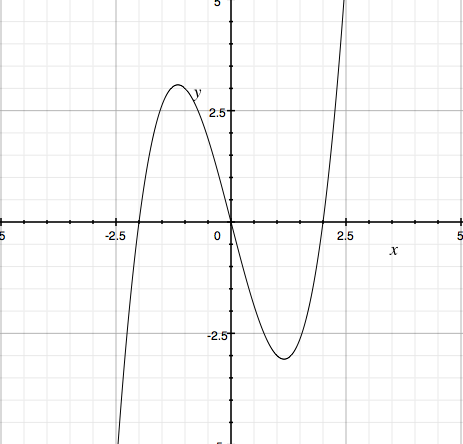
\includegraphics[scale=0.5]{graph_a}
\caption{An example graph}
\label{fig:x cubed graph}
\end{figure}


\subsection{SubSection Title}


\subsection{SubSection Title}


\chapter{Chapter Three Title}
\section{Section Title}


\begin{figure}
    \centering
    \begin{subfigure}[b]{0.3\textwidth}
        \centering
        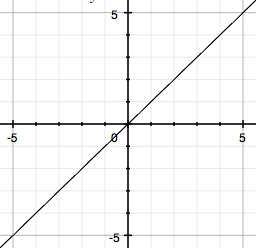
\includegraphics[width=\textwidth]{graph1}
        \caption{$y=x$}
        \label{fig:y equals x}
    \end{subfigure}
    \hfill
    \begin{subfigure}[b]{0.3\textwidth}
        \centering
        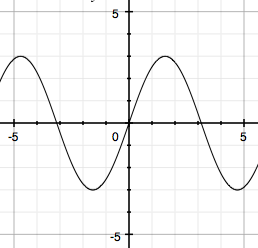
\includegraphics[width=\textwidth]{graph2}
        \caption{$y=3sinx$}
        \label{fig:three sin x}
    \end{subfigure}
    \hfill
    \begin{subfigure}[b]{0.3\textwidth}
        \centering
        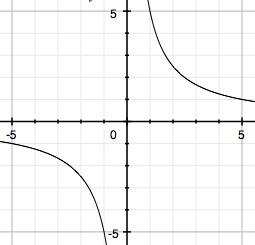
\includegraphics[width=\textwidth]{graph3}
        \caption{$y=5/x$}
        \label{fig:five over x}
    \end{subfigure}
    \caption{Three simple graphs}
    \label{fig:three graphs}
\end{figure}



\subsection{SubSection Title}


\chapter{Chapter Four Title}
\section{Section Title}


\begin{table}[h]
\centering
\begin{tabular}{l | l | l}
A & B & C \\
\hline
1 & 2 & 3 \\
4 & 5 & 6
\end{tabular}
\caption{very basic table}
\label{tab:abc}
\end{table}


\section{Section Title}

\section{Section Title}

\begin{table}[h]
    \begin{subtable}[h]{0.45\textwidth}
        \centering
        \begin{tabular}{l | l | l}
        Day & Max Temp & Min Temp \\
        \hline \hline
        Mon & 20 & 13\\
        Tue & 22 & 14\\
        Wed & 23 & 12\\
        Thurs & 25 & 13\\
        Fri & 18 & 7\\
        Sat & 15 & 13\\
        Sun & 20 & 13
        \end{tabular}
        \caption{First Week}
        \label{tab:week1}
    \end{subtable}
    \hfill
    \begin{subtable}[h]{0.45\textwidth}
        \centering
        \begin{tabular}{l | l | l}
        Day & Max Temp & Min Temp \\
        \hline \hline
        Mon & 17 & 11\\
        Tue & 16 & 10\\
        Wed & 14 & 8\\
        Thurs & 12 & 5\\
        Fri & 15 & 7\\
        Sat & 16 & 12\\
        Sun & 15 & 9
        \end{tabular}
        \caption{Second Week}
        \label{tab:week2}
    \end{subtable}
    \caption{Max and min temps recorded in the first two weeks of July}
    \label{tab:temps}
\end{table}


\chapter{Conclusion}
\input{chapters/conclusion}

\appendix   %all chapters after this command will be appendices
\chapter{Appendix Title}
Appendix goes here...

%references. use bibtex file
\bibliography{references}{}
%\bibliographystyle{plain}


\end{document}
